\chapter{Face authentication}
    Face recognition is a problem that has been around for a while and
    human-level solutions have been developed, such as FaceNet \cite{arXiv:1503.03832}.
    However, there are many subtleties to face recognition in mobile devices
    security, in particular when using unconventional cameras.

    From the security context, false positives are very problematic. This observation alone
    poses two questions:
    \begin{itemize}
      \item How to measure a model's performance to punish false positives?
      \item How to maximize our chosen score measure?
    \end{itemize}
    We have tackled two problems in our research -- multi-class and binary classification.
    Binary classification is more adequate to the possible applications of our research.
    Multi-class classification allows the reader to compare the achieved results
    with other face recognition models.

    The second observation is more optimistic: the front camera of a mobile is capable of
    capturing relatively many frames per second. We decided not to constrain our
    methods to a classification based on a single frame.
    Moreover, a large training set can be built
    when adding a new user to the device -- it is not unreasonable to make that procedure
    longer for increased security. We aimed to take advantage of those factors.

    \section{Data set}
    We have set requirements for our dataset, aiming to reflect real-life
    appliances:
    \begin{itemize}
        \item \textbf{depth and IR channels}: in real-life appliance, leveraging
        the infrared camera allows equally good vision regardless of lighting
        conditions.
        \item \textbf{various vertical angles}: when a user is looking at their
        mobile device,
        their head may be placed at various angles along the vertical axis.
        However, it is reasonable to assume that the angle along the horizontal
        axis will be small, especially if the user is consciously trying to
        unlock the device.
        \item \textbf{many frames per subject}: when a new user is being added
        to a mobile device's authentication system, it is acceptable to require
        them to look at the camera, at various angles, for a short period of
        time. Many frames can (and should) be taken.
    \end{itemize}

    There are several good databases for face recognition with depth camera:
    The EURECOM Kinect Face Database \cite{eurecom},
    RGB-D Face database \cite{vapaaudk},
    The Florence Superface dataset \cite{superface}. However, none of them was
    deemed suiting for our project, primarily due to the lack of IR channel.
    Thus, we have decided to build a dedicated dataset.

    \subsection*{Data collection}

    \subsubsection*{Hardware, libkinect}
    For this project, we had one Kinect v1 camera and two Kinect v2 cameras.
    Because we use Linux, we could not use Microsoft's API for Kinects and decided to
    use open source libraries: \texttt{libfreenect} \cite{libfreenect}
    and \texttt{libfreenect2} \cite{libfreenect2} developed by the OpenKinect community.

    Since our team had four members, we could not always have the same Kinects available
    for everyone, and sometimes one person would need to use Kinect v1 and another one
    Kinect v2 to run the same program.
    That is why we decided to create \texttt{libkinect}, which is a library that
    gives a simple interface for receiving images from a Kinect camera
    regardless of its version, allowing the programmer to focus on important code
    and not making the Kinect work.

    Based on \texttt{libkinect} and its file format for depth and IR photos,
    we made a program that displayed live video from the connected Kinect device
    and allowed saving received frames, a program that displayed a file
    and a thumbnailer that can be configured to show thumbnails of depth and IR photos
    in graphical file managers.

    \begin{figure}[H]
        \centering
        \caption{Screenshots of implemented tools}
        \begin{subfigure}[b]{0.49\textwidth}
            \caption{Live Kinect display}
            \centering
            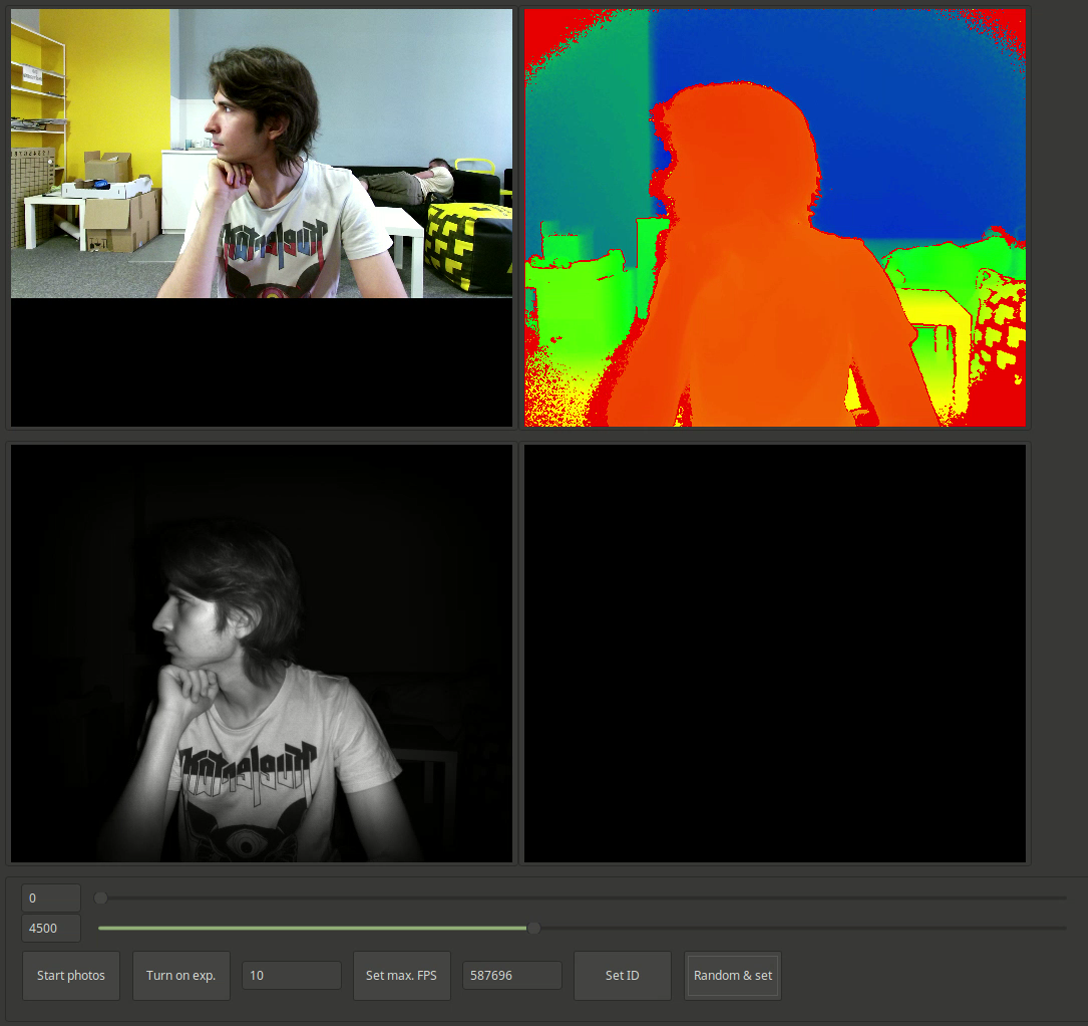
\includegraphics[height=7cm]{libkinect_live_display}
        \end{subfigure}
        \begin{subfigure}[b]{0.49\textwidth}
            \caption{Depth file display}
            \centering
            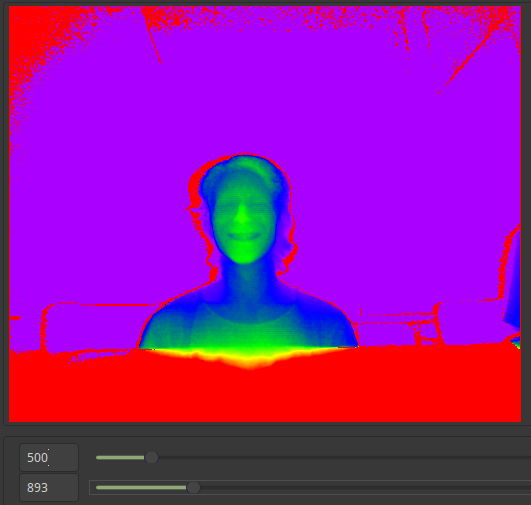
\includegraphics[height=7cm]{libkinect_file_display}
        \end{subfigure}\\
        \vspace{3mm}
        \begin{subfigure}[b]{0.6\textwidth}
            \caption{Thumbnails in Nemo file manager}
            \centering
            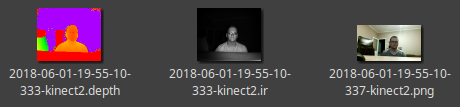
\includegraphics[width=\textwidth]{libkinect_thumbnails}
        \end{subfigure}
        \label{fig:libkinect_screenshots}
    \end{figure}

    Both the live and file display programs allowed setting a scale for applying the color
    map to the depth image. On \ref{fig:libkinect_screenshots}.a) the interval of shown
    depth values is very high, so objects in the background are visible, but it is not
    possible to see any details on the face. On \ref{fig:libkinect_screenshots}.b)
    face details are clearly visible because the interval is much smaller.

    Other features of the live display program included:
    \begin{itemize}
        \item Limiting frames per second while maintaining synchronization
        between depth and infrared frames -- we did not want to collect photos at 30 FPS,
        because that would take too much disk space while not adding too much new
        information.
        \item Saving received frames to hard drive.
        \item Quickly changing the directory of saved photos to allow easy distinction
        between different volunteers.
        \item A fourth display, black on the screenshot, on which we could display
        experiments such as on figure \ref{fig:skin_kinect_2}.
    \end{itemize}


    \subsubsection*{Details of our dataset}
    The dataset consists of $44$ subjects: $36$ males and
    $8$ females, mostly aged $20$-$25$. Each subject has been asked to
    follow an object with their entire head, making two cycles of slow,
    continuous movements: \texttt{up $\to$ center $\to$ down $\to$ center $\to$
    left $\to$ center $\to$ right $\to$ center}.
    That procedure has resulted in approximately $20$ seconds of footage per
    subject.

    IR and depth frames are synchronized, taken at $10$ FPS rate.

    We used only Kinect v2 cameras, because they give more detailed depth pictures
    than Kinect v1, and its infrared images do not have a dotted pattern,
    which is projected by Kinect v1 because it uses a different depth
    measurement method.

    Dataset contains also RGB frames taken at $10$ FPS rate, not synchronized
    with IR and depth frames.

    The procedure performed to collect photos of a single person took around $20$-$30$ seconds.
    We believe it could be proposed as a part of mobile device's first time security configuration.

    \subsection*{Test set}
    For the test set, we have chosen approximately first $25\%$ of
    frames from each subject -- the first two vertical head rotations.
    \newpage

    \subsection*{Samples}
    \begin{figure}[H]
    \caption{One of the subjects from the database -- the first $269$ IR frames.}
    \centering
    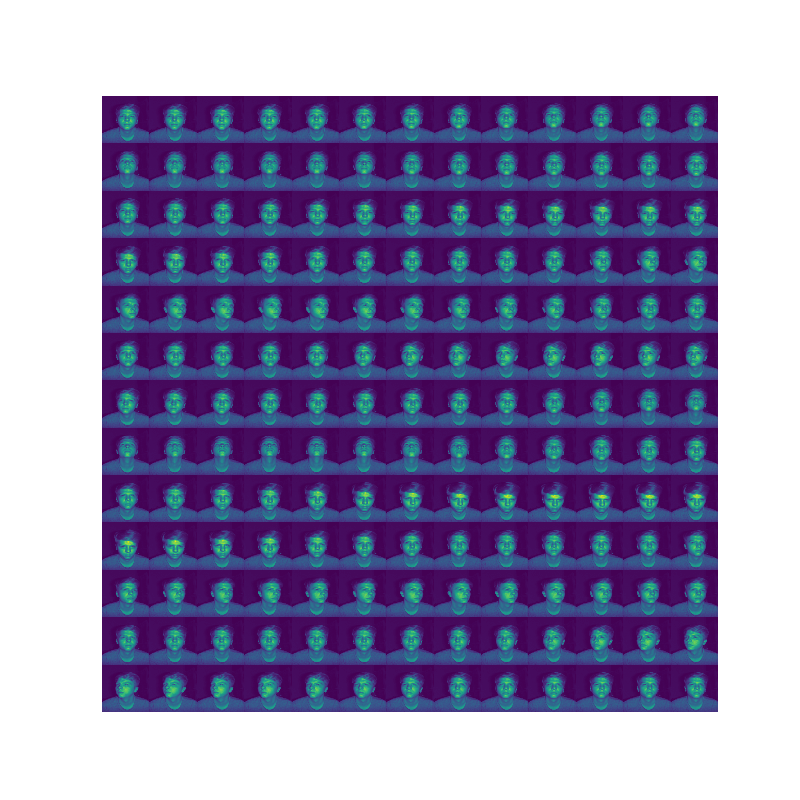
\includegraphics[scale=0.5]{tiled_faces_ludziej}
    \end{figure}

    \section{Face angle detection}
    \label{sec:angledetection}
    Using depth camera, we can extract more structural features of an image,
    and normalize the face angle. Face is positioned in a cube, and position vector is computed
    by finding three points located on face, describing the surface
    and computing its orthogonal vector. We define face position
    as the angle between the computed vector and vector $[0,0,1]^T$ pointing towards the camera.
    We have chosen the points as the middle of each eyebrow and the middle of the chin and compute them with
    same library we use for face trimming (as an average between chosen subsets of points). Worth
    mentioning is that choosing points too close to the edge of face (as most algorithms do)
    detected on 2-dimensional image, might turn algorithm unstable, because small error can place the point on the background,
    far away in third dimension.


    \begin{figure}[H]
    \caption{Detecting the angle of face. The face orthogonal vector is positioned between eyebrows, face points are marked yellow}
    \centering
    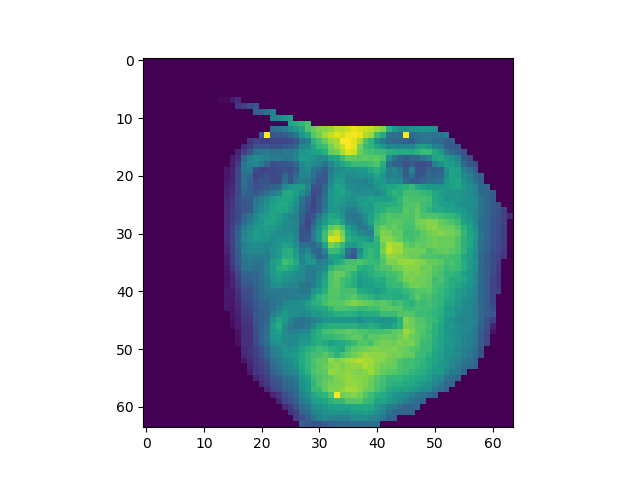
\includegraphics[scale=0.3]{angle}
    \end{figure}


    \section{Normalization}
        \subsection*{Depth mean and standard deviation normalization}
        Let $F$ be the set of all points belonging to the trimmed face and
        $d(p)$ -- depth of the point $p$. Let $\mu$ denote the mean depth, i.e.
        $\mu = \frac{\sum\limits_{p \in F}{d(p)}}{|F|}$ and $\sigma$ -- standard
        deviation, i.e. $\sigma = \sqrt{\frac{1}{|F|} \sum\limits_{p \in F}{(d(p) - \mu)^2}}$.
        For each pixel $p$, its new depth is calculated as:

        \begin{center}
        $
          d'(p) = \begin{cases}
                  d(p) - \mu &\quad\text{if}\ |d(p) - \mu| \leqslant 2 \cdot \sigma \\
                  0 &\quad\text{otherwise}
                  \end{cases}
        $
        \end{center}


        Lastly, all depth values are scaled to the interval $[0..1]$:
        \begin{center}
        $
          d''(p) = \frac{d'(p) - min(\{d'(r)\ |\ r \in F\})}{max(\{d'(r)\ |\ r \in F\}) - min(\{d'(r)\ |\ r \in F\})}
        $
        \end{center}

        \subsection*{Face angle normalization}
        Depth channel provides substantial information about faces' geometry, thus allowing
        a meaningful normalization method -- rotation to the frontal position.

        With our ability to detect face angle (\ref{sec:angledetection}), we can obtain
        three values: $\theta_x, \theta_y, \theta_z$ -- angles along each axis.

        The face can be represented as a cloud of $3$-dimensional, "colorful" points.
        Point $p$ is defined as a vector $[x_p, y_p, z_p, ir_p]^{T}$.

        Let $R_x(\theta_x), R_y(\theta_y), R_z(\theta_z)$ denote the rotation matrices
        for $X, Y, Z$ axes, as follows:
        \[
        R_x(\theta_x) =
        \begin{bmatrix}
        1 & 0 & 0\\
        0 & cos(\theta_x) & -sin(\theta_x)\\
        0 & sin(\theta_x) & cos(\theta_x)
        \end{bmatrix}
        \]
        \[
        R_y(\theta_y) =
        \begin{bmatrix}
        cos(\theta_y) & 0 & sin(\theta_y)\\
        0 & 1 & 0\\
        -sin(\theta_y) & 0 & cos(\theta_y)
        \end{bmatrix}
        \]
        \[
        R_z(\theta_z) =
        \begin{bmatrix}
        cos(\theta_z) & -sin(\theta_z) & 0\\
        sin(\theta_z) & cos(\theta_z) & 0\\
        0 & 0 & 1
        \end{bmatrix}
        \]
        The operation of rotating a single point is a product of its coordinates and the three rotation matrices:
        \begin{center}
        $
        \begin{bmatrix}
          x_p\\
          y_p\\
          z_p\\
          ir_p
        \end{bmatrix}
        \cdot
        \begin{bmatrix}
          R_x & 0_{3}^T\\
          0_{3} & 1
        \end{bmatrix}
        \cdot
        \begin{bmatrix}
          R_y & 0_{3}^T\\
          0_{3} & 1
        \end{bmatrix}
        \cdot
        \begin{bmatrix}
          R_z & 0_{3}^T\\
          0_{3} & 1
        \end{bmatrix}
        $
        \end{center}

        Face angle normalization was implemented with smaller datasets in mind
        (\cite{eurecom}, \cite{vapaaudk}). Our final training set
        contains many different angles of each face, rendering this technique obsolete.
        In our final models we have not used it.

        \begin{figure}[H]
        \caption{Face from angle detection subsection, transformed.}
        \centering
        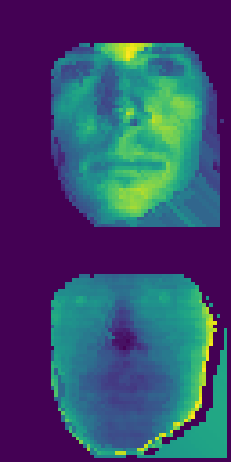
\includegraphics[scale=0.3]{angle_transformed}
        \end{figure}

    \section{Preprocessing techniques}
    We have used several different preprocessing techniques.
        \subsection*{Trimming faces}
        \label{sec:trimming}
        During the process of collecting the dataset, each subject has been
        recorded in only one set of clothes (the ones they were wearing at the
        time), one hairstyle and the background may slightly vary among the
        subjects (the background behind subjects recorded at $12$ a.m. is
        likely to be brighter than behind the subjects recorded at $4$ p.m.
        Additionally, there are $4$ different backgrounds in our dataset).

        Since a classifier might leverage those factors, photos have been
        trimmed to polygons containing the faces. Such polygons have been
        found with Face Recognition library \cite{facerecog} on IR photos.
        Depth photos have been trimmed accordingly.

        \begin{figure}[H]
        \caption{Before and after trimming the face.}
        \centering
        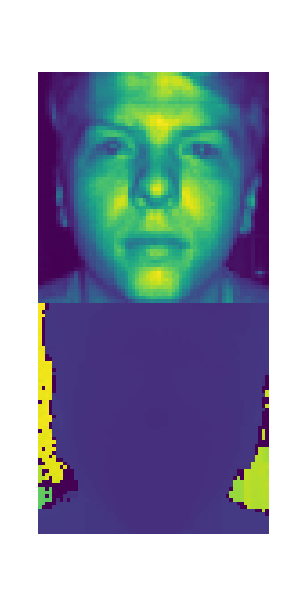
\includegraphics[scale=0.25]{before_trim_ludziej}
        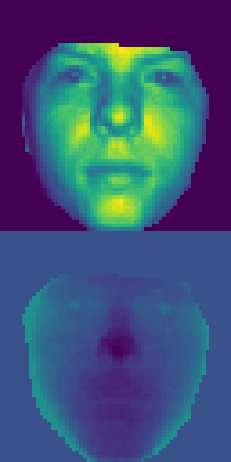
\includegraphics[scale=0.25]{after_trim_ludziej}
        \end{figure}

        \subsection*{HOGs}
        To transform 2-dimensional images into 1-dimensional feature descriptors,
        we used standard preprocessing called Histogram of Oriented Gradients, commonly used in
        object detection (\citeauthor{hog}), purposely to ensemble 1-dimensional classifier with CNN,
        as different techniques achieve better results together. Briefly describing,
        HOGs divide image into cells, and then count gradient occurrences in each one.
        Recently, this technique alone has achieved sensible results in face detection using depth camera (\citeauthor{rgbdhog}).

        \subsection*{Entropy maps}
        To exctract meaningful information (as \citeauthor{rgbdhog}),
        we used entropy maps, to amplify small variations on depth images, and provide
        more information to classifiers.

        \subsection*{Channels vs concatenation}
        A choice of the input format passed to a classifier is not only a matter
        of images to include. Another decision to be made is whether different
        channels (IR, depth) and different preprocessed images (entropy maps,
        HOGs) should be concatenated or layered as channels. In our experiments,
        we have included both approaches, although channels quickly proved to
        give better results.

        \subsection*{Data augmentation}
        To further enhance the training set, we have used image augmentations, with \texttt{imgaug} \cite{imgaug} library.
        The used transformations include:
        \begin{itemize}
            \item \textbf{coarse salt and pepper} -- randomly placed patches of grain (black and white pixels)
            \item \textbf{padding} -- shifting the input image $3$ pixels in random direction
            \item \textbf{Gaussian blur} with several different strenghts
            \item \textbf{rotations} by $2$ degrees
            \item \textbf{PiecewiseAffine} -- augmenter that places a regular grid of points on an image and randomly moves the neighbourhood of these point around via affine transformations.
        \end{itemize}
        \begin{figure}[H]
        \caption{Trimming + all possible augmentations.}
        \centering
        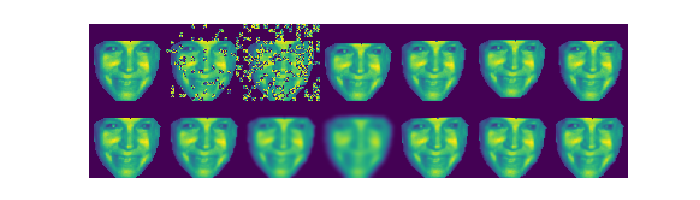
\includegraphics[scale=0.5]{augmenters}
        \end{figure}

    \section{Classifiers}
        \subsection{Convolutional Neural Network}
        We have used a convolutional neural network with the following structure:
        \begin{itemize}
            \item \textbf{Layers}:
            \begin{itemize}
            \item[$\blacksquare$] \textbf{conv. layer 0}: $20$ filters, $5 \text{x} 5$ kernel
            \item[$\blacksquare$] \textbf{max pooling}: $2 \text{x} 2$ pool size, $2 \text{x} 2$ strides
            \item[$\blacksquare$] \textbf{conv. layer 1}: $20$ filters, $5 \text{x} 5$ kernel
            \item[$\blacksquare$] \textbf{max pooling}: $2 \text{x} 2$ pool size, $2 \text{x} 2$ strides
            \item[$\blacksquare$] \textbf{conv. layer 2}: $40$ filters, $5 \text{x} 5$ kernel
            \item[$\blacksquare$] \textbf{max pooling}: $2 \text{x} 2$ pool size, $2 \text{x} 2$ strides
            \item[$\blacksquare$] \textbf{dense layer} with sigmoid activation function
            \end{itemize}
            \item \textbf{Loss function}: Log Loss
            \item \textbf{Optimizer}: SGD
            \item \textbf{Kernels initialization}: Since we have experimented with deeper
            networks too, and each model was trained from scratch, a reckless initialization
            would hamper the models ability to learn and increase the number of
            iterations needed for convergence. To ensure quick start of the learning
            process, we decided to initialize each kernel with \textbf{random normal
            distribution with $\mu = 0,\ \sigma = \sqrt{(2 / N)}$}, as advised by
            \citeauthor{initialization}.
        \end{itemize}


        \begin{figure}[H]
        \caption{Convolved input images (only IR channel). First two rows
        are outputs from first and second convolutional layers. Third and fourth
        row are outputs from all $40$ filters from last convolutional layer.
        }
        \centering
        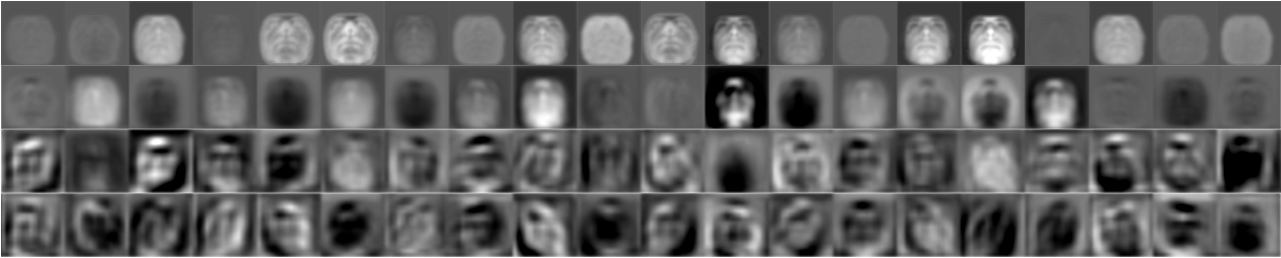
\includegraphics[scale=0.25]{convolutions}
        \end{figure}
        \begin{figure}[H]
            \caption{For each filter in each convolutional layer, $10$ patches
            among one of the test batches were chosen that activate those
            filters the most.
            Horizontally, consecutive filters are presented, vertically -- patches
            sorted from the highest activation.
            Note that from each patch, only IR channel is presented.
            }
            \centering
            \begin{subfigure}[b]{0.4\textwidth}
                \centering
                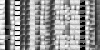
\includegraphics[scale=0.28]{exciting_layer0}
                \caption{conv. layer 0}
            \end{subfigure}
            \begin{subfigure}[b]{0.4\textwidth}
                \centering
                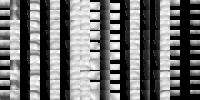
\includegraphics[scale=0.14]{exciting_layer1}
                \caption{conv. layer 1}
            \end{subfigure}
            \\
            \begin{subfigure}[b]{0.8\textwidth}
                \centering
                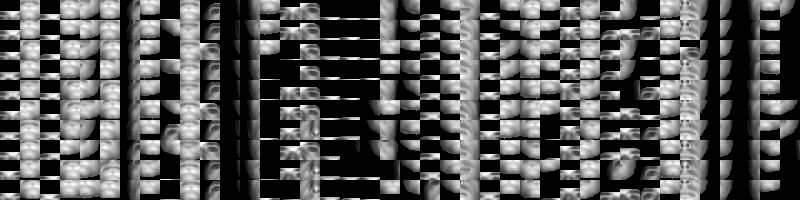
\includegraphics[scale=0.35]{exciting_layer2}
                \caption{conv. layer 2}
            \end{subfigure}
        \end{figure}

        \subsection{HOG + SVM}
        As an alterative to CNN, to classify HOG feature descriptors, we tested two common (\citeauthor{hog}, \citeauthor{rgbdhog}) approaches:
        Support Vector Machine, extremely randomised decision trees (Extra Trees), and both ensembled.
        Initially, while collecting the data and working with smaller dataset, Extra Trees where achieving higher results,
        and SVM was highly overfitting, but as the work proceeded, the second approach was getting better and has finally overcome Extra Trees
        to the point that the other classifier was not even contributing to ensembling, so further work was continued only with Support Vector Machines.
        In multi-class classification, we used One vs Rest approach.

        After tuning the parameters on final dataset using grid-search approach, the following configuration of most important parameters was chosen:
        \begin{itemize}
            \item \textbf{Polynomial kernel} with degree 3. Other kernels got significantly worse results.
            \item \textbf{Penalty C parameter}: 10, locally constant results results in range [1, 10].
            \item \textbf{Gamma parameter}: 0.7, locally constant results results in range [0.1, 1].
        \end{itemize}

        \subsection{Ensembling}
        We have experimented with a simple ensembling method -- voting.
        Each of our classifiers is implemented in a way that allows getting,
        apart from predictions, a vector of probabilities for each class.

        Let $C^{(1)}, C^{(2)}$ be two classifiers running in the same mode -- either
        binary or multi-class.
        Let $p_{C}(f)$ denote predicted probabilities for each class by classifier $C$,
        given input $f$.

        An ensembling classifier is configured by two values $w_1, w_2$ -- significance
        weights for classifiers $C^{(1)}, C^{(2)}$. Its output for input $f$ is defined as:
        \begin{center}
        $C_{E}(f) = \frac{w_{1} \cdot p_{C^{(1)}}(f) + w_{2} \cdot p_{C^{(2)}}(f)}{w_{1} + w_{2}}$
        \end{center}

        We will use notation $C^{(1)}\ w_{1}\ :\ w_{2}\ C^{(2)}$ to denote ensembling
        of classifiers $C^{(1)}$ and $C^{(2)}$ with weights $w_{1}, w_{2}$f.


    \section{Quality measures}
        Models have been trained in two modes: multi-class and binary
        classification. Let $T$ be the test set, $p_t$ -- predictions for test input
        $t \in T$ and $y_t$ -- ground truth for test input $t \in T$.
        \subsection*{Accuracy}
        For classifiers trained in multi-class mode the accuracy score has been
        measured:

        \begin{center}
        $acc(p, y) = \frac{|\{t \in T\ |\ p_t = y_t\}|}{|T|}$
        \end{center}

        \subsection*{Recall for fixed precision}

        When testing the model in binary mode two decisions are being made:
        \begin{itemize}
            \item \textbf{positive class (device owner)}: One subject from the
            database is chosen as the "device owner". All photos of this subjects
            are then labeled as positive. All photos of other subjects are
            labeled as negative.
            \item \textbf{desired precision threshold:}
            Precision is defined as:
            \begin{center}
            $prec(p, y) = \frac{\{t \in T\ |\ y_t = p_t = 1\}}{\{t \in T\ |\ p_t = 1\}}$
            \end{center}
            We have chosen $3$ different precision thresholds: $0.99$, $0.999$, $0.9999$.
        \end{itemize}
        Recall is defined as:
        \begin{center}
        $rec(p, y) = \frac{\{t \in T\ |\ p_t = y_t = 1\}}{\{t \in T\ |\ y_t = 1\}}$
        \end{center}
        For each precision threshold, we have calculated the corresponding recall measure and
        averaged the result over $5$ random choices for positive class.

    \begin{figure}[H]
    \caption{Test samples misclassified by CNN}
    \centering
    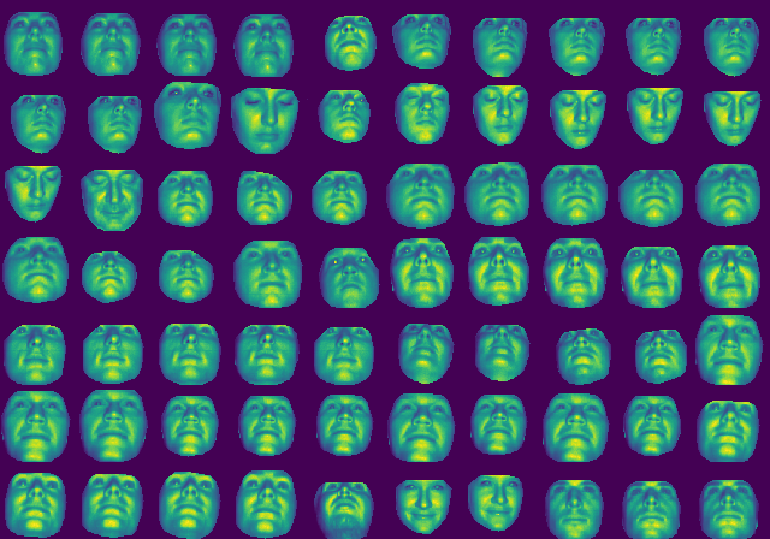
\includegraphics[scale=0.4]{misclassified}
    \end{figure}


    \section{Single-frame model results}
        We call a model single-frame if it classifies the person on the photo
        using only one frame. We have evaluated several single-frame models to
        choose one multi-class and one binary classifier.
        \subsection{Multi-class}
        \begin{table}[H]
        \begin{center}
        \small
        \caption{Selected models performance in multi-class mode}
        \begin{tabular}{ |c|c|c| }
            \hline
            Model & CNN inputs & Accuracy\\
            \hline
            CNN & channels & 0.9721\\
            \hline
            CNN 10 : 1 SVM + HOGs & channels & 0.9721\\
            \hline
            CNN 2 : 1 SVM + HOGs & channels & 0.9648\\
            \hline
            CNN 10 : 7 SVM + HOGs & channels & 0.9631\\
            \hline
            CNN 1 : 2 SVM + HOGs & channels & 0.9536\\
            \hline
            SVM + HOGs & - & 0.9099\\
            \hline
            CNN & concat & 0.8899\\
            \hline
        \end{tabular}
        \end{center}
        \end{table}

        \subsection{Binary}
        \begin{table}[H]
        \begin{center}
        \small
        \caption{Selected models performance in binary mode}
        \begin{tabular}{ |c|c|c|c| }
            \hline
            Model & CNN input & Precision & Recall\\
        \hline
        CNN 1 : 5 SVM + HOGs & channels & 0.99 & 0.9079\\
        & & 0.999 & 0.9013\\
        & & 0.9999 & 0.9013\\
        \hline
        SVM + HOGs & - & 0.99 & 0.8947 \\
        & & 0.999 & 0.8947\\
        & & 0.9999 & 0.8947\\
        \hline
        CNN & channels & 0.99 & 0.8487 \\
        & & 0.999 & 0.8487\\
        & & 0.9999 & 0.8487\\
        \hline
        CNN 1 : 1 SVM + HOGs & channels & 0.99 & 0.6908\\
        & & 0.999 & 0.6777\\
        & & 0.9999 & 0.6777\\
        \hline

        \end{tabular}
        \end{center}
        \end{table}

    \section{Multiple frames based classification}
    We have chosen CNN as multi-class classifier and CNN ensembled with SVM (CNN 1 : 5 SVM) as
    best performing single-frame classifiers.

    \subsection{Generating predictions from multiple frames}
    Let $n$ be the number of frames, $C_{1}$ -- a single-frame classifier and
    $f_1, ..., f_n$ be the $n$ consecutive frames.
    Let $p_{C_{1}}(f)$ denote the vector of probabilities predicted for each class by $C_{1}$,
    with frame $f$ as input.

    Note that $p_{C_{1}}(f) \in [0..1]^D$ where $D = 1$ for binary classification
    and $D$ equals to the number of classes in multi-class mode -- in our case $D = 44$.


    The multi-frame classifier $C_{n}$ can be defined as a function (namely arithmetic mean)
    from a tuple of $n$ frames to the vector of predicted probabilities:

    \begin{center}
    $C_{n}(f_1, ..., f_n) = \frac{\sum\limits_{i=1}^{n}{p_{C_{1}}(f_{i})}}{n}$
    \end{center}

    Another way of looking at multiple frames based classifier is as an ensembling
    of $n$ identical classifiers, but each receives a different frame as an input.
    \newpage

    \subsection{Results -- multi-class}

    \begin{figure}[H]
        \caption{Frames-accuracy relation for multiclass problem}
        \centering
        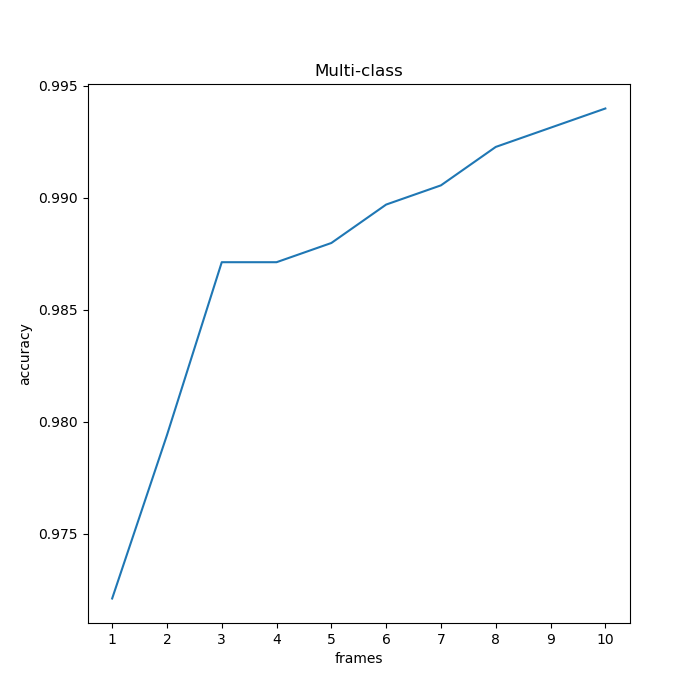
\includegraphics[scale=0.5]{multiclass_frames_accuracy_relation}
    \end{figure}

    \begin{table}[H]
      \begin{center}
      \small
      \caption{Accuracy obtained by multi-frame based classification with CNN}
      \begin{tabular}{ |c|c| }
      \hline
      Frames & Accuracy\\
      \hline
      1 & 0.9721\\
      \hline
      2 & 0.9794\\
      \hline
      3 & 0.9871\\
      \hline
      4 & 0.9871\\
      \hline
      5 & 0.9879\\
      \hline
      6 & 0.9896\\
      \hline
      7 & 0.9905\\
      \hline
      8 & 0.9922\\
      \hline
      9 & 0.9931\\
      \hline
      10 & 0.9940\\
      \hline
      \end{tabular}
      \end{center}
    \end{table}
    \newpage

    \subsection{Results -- binary}

    \begin{figure}[H]
        \centering
        \caption{Frames-accuracy relation for binary problem}
        \begin{subfigure}[b]{0.48\textwidth}
            \raggedleft
            \caption{Precision threshold $\geqslant 0.99$}
            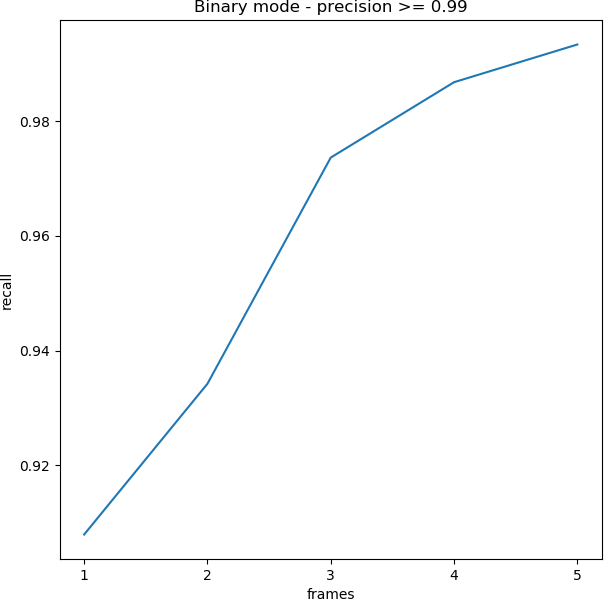
\includegraphics[width=\textwidth]{binary_frames_recall_relation_099}
        \end{subfigure}
        \hspace*{\fill}
        \begin{subfigure}[b]{0.48\textwidth}
            \raggedright
            \caption{Precision threshold $\geqslant 0.999$}
            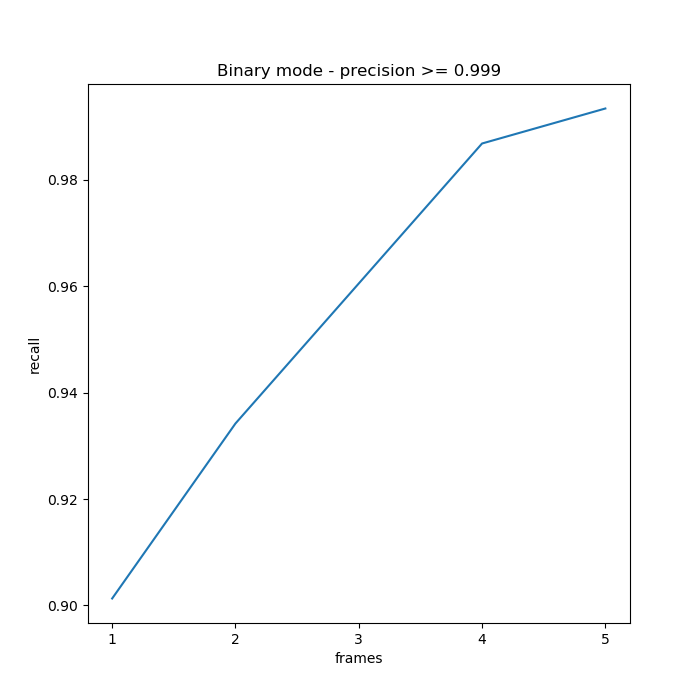
\includegraphics[width=\textwidth]{binary_frames_recall_relation_0999}
        \end{subfigure}\\
        \vspace{5mm}
        \begin{subfigure}[b]{0.48\textwidth}
            \centering
            \caption{Precision threshold $\geqslant 0.9999$}
            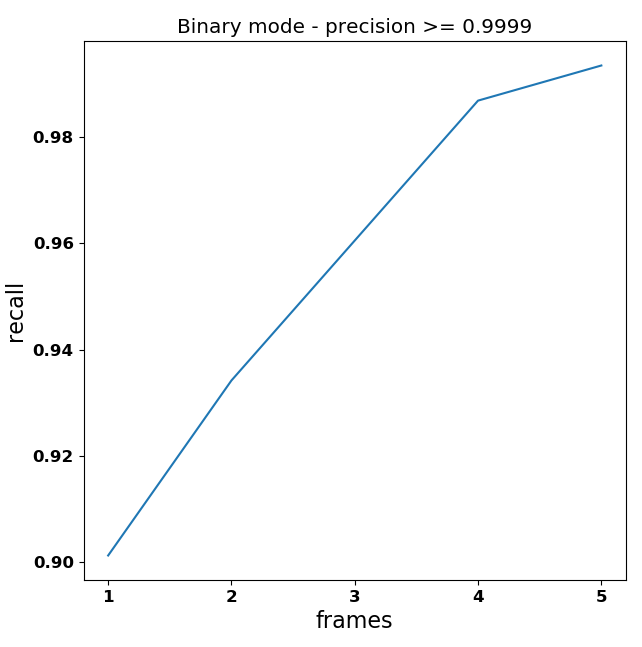
\includegraphics[width=\textwidth]{binary_frames_recall_relation_09999}
        \end{subfigure}
    \end{figure}
    \newpage


    \begin{table}[H]
    \begin{center}
    \small
    \caption{Recall obtained by multi-frame based classification with CNN 1 : 5 SVM}
    \begin{tabular}{ |c|c|c| }
        \hline
        Frames & Precision & Recall\\
    \hline
    1 & 0.99 & 0.9079\\
    & 0.999 & 0.9013\\
    & 0.9999 & 0.9013\\
    \hline
    2 & 0.99 & 0.9342\\
    & 0.999 & 0.9342\\
    & 0.9999 & 0.9342\\
    \hline
    3 & 0.99 & 0.9736\\
    & 0.999 & 0.9605\\
    & 0.9999 & 0.9605\\
    \hline
    4 & 0.99 & 0.9868\\
    & 0.999 & 0.9868\\
    & 0.9999 & 0.9868\\
    \hline
    5 & 0.99 & 0.9934\\
    & 0.999 & 0.9934\\
    & 0.9999 & 0.9934\\
    \hline

    \end{tabular}
    \end{center}
    \end{table}

    \section*{Possible improvements}

    \subsection*{Not tested approach to multi-frame classification}
    Instead of implementing multiple frame based classification as an ensembling
    of several single-frame classifiers, a single classifier could also be used.
    We believe that a recurrent neural network (RNN) might be a good fit for the
    task.

    \subsection*{Speed optimization}
    In our experiments, an external, heavy duty machine learning-based library
    has been used for finding and trimming faces (\ref{sec:trimming}). This has
    resulted in a single frame classification time of $260$ miliseconds -- most of
    which spent on detecting and trimming the face. This is too slow for $10$ FPS
    rate.

    We believe that a fully developed skin-recognition method, possibly with
    additional infrared channels on different wavelengths, could replace the
    all-in-one face detection library. Unfortunately, due to hardware limitations,
    we were unable to verify this assumption in our research.

    \section{Proposed solution}
    The solution we propose is a voting ensembling CNN 1 : 5 SVM, with
    classification based on $4$ consecutive frames. We believe that $400$ miliseconds
    is an acceptable authentication time. Using $4$ frames, precision rate $0.9999$
    and recall rate $0.9868$ are achievable.

    In other words, our solution will fail to protect users resources or device
    only once in $10\ 000$ cases. Out of $10\ 000$ cases when the right owner
    tries to access the device or resources, only $132$ times they will fail
    to authorize.
